\documentclass[a4paper,12pt,twoside]{memoir}

% Castellano
\usepackage[spanish,es-tabla]{babel}
\selectlanguage{spanish}
\usepackage[utf8]{inputenc}
\usepackage[T1]{fontenc}
\usepackage{lmodern} % scalable font
\usepackage{microtype}
\usepackage{placeins}

\RequirePackage{booktabs}
\RequirePackage[table]{xcolor}
\RequirePackage{xtab}
\RequirePackage{multirow}

% Links
\usepackage[colorlinks]{hyperref}
\hypersetup{
	allcolors = {red}
}

% Ecuaciones
\usepackage{amsmath}

% Rutas de fichero / paquete
\newcommand{\ruta}[1]{{\sffamily #1}}

% Párrafos
\nonzeroparskip


% Imagenes
\usepackage{graphicx}
\newcommand{\imagen}[2]{
	\begin{figure}[!h]
		\centering
		\includegraphics[width=0.9\textwidth]{#1}
		\caption{#2}\label{fig:#1}
	\end{figure}
	\FloatBarrier
}

\newcommand{\imagenflotante}[2]{
	\begin{figure}%[!h]
		\centering
		\includegraphics[width=0.9\textwidth]{#1}
		\caption{#2}\label{fig:#1}
	\end{figure}
}



% El comando \figura nos permite insertar figuras comodamente, y utilizando
% siempre el mismo formato. Los parametros son:
% 1 -> Porcentaje del ancho de página que ocupará la figura (de 0 a 1)
% 2 --> Fichero de la imagen
% 3 --> Texto a pie de imagen
% 4 --> Etiqueta (label) para referencias
% 5 --> Opciones que queramos pasarle al \includegraphics
% 6 --> Opciones de posicionamiento a pasarle a \begin{figure}
\newcommand{\figuraConPosicion}[6]{%
  \setlength{\anchoFloat}{#1\textwidth}%
  \addtolength{\anchoFloat}{-4\fboxsep}%
  \setlength{\anchoFigura}{\anchoFloat}%
  \begin{figure}[#6]
    \begin{center}%
      \Ovalbox{%
        \begin{minipage}{\anchoFloat}%
          \begin{center}%
            \includegraphics[width=\anchoFigura,#5]{#2}%
            \caption{#3}%
            \label{#4}%
          \end{center}%
        \end{minipage}
      }%
    \end{center}%
  \end{figure}%
}

%
% Comando para incluir imágenes en formato apaisado (sin marco).
\newcommand{\figuraApaisadaSinMarco}[5]{%
  \begin{figure}%
    \begin{center}%
    \includegraphics[angle=90,height=#1\textheight,#5]{#2}%
    \caption{#3}%
    \label{#4}%
    \end{center}%
  \end{figure}%
}
% Para las tablas
\newcommand{\otoprule}{\midrule [\heavyrulewidth]}
%
% Nuevo comando para tablas pequeñas (menos de una página).
\newcommand{\tablaSmall}[5]{%
 \begin{table}
  \begin{center}
   \rowcolors {2}{gray!35}{}
   \begin{tabular}{#2}
    \toprule
    #4
    \otoprule
    #5
    \bottomrule
   \end{tabular}
   \caption{#1}
   \label{tabla:#3}
  \end{center}
 \end{table}
}

%
%Para el float H de tablaSmallSinColores
\usepackage{float}

%
% Nuevo comando para tablas pequeñas (menos de una página).
\newcommand{\tablaSmallSinColores}[5]{%
 \begin{table}[H]
  \begin{center}
   \begin{tabular}{#2}
    \toprule
    #4
    \otoprule
    #5
    \bottomrule
   \end{tabular}
   \caption{#1}
   \label{tabla:#3}
  \end{center}
 \end{table}
}

\newcommand{\tablaApaisadaSmall}[5]{%
\begin{landscape}
  \begin{table}
   \begin{center}
    \rowcolors {2}{gray!35}{}
    \begin{tabular}{#2}
     \toprule
     #4
     \otoprule
     #5
     \bottomrule
    \end{tabular}
    \caption{#1}
    \label{tabla:#3}
   \end{center}
  \end{table}
\end{landscape}
}

%
% Nuevo comando para tablas grandes con cabecera y filas alternas coloreadas en gris.
\newcommand{\tabla}[6]{%
  \begin{center}
    \tablefirsthead{
      \toprule
      #5
      \otoprule
    }
    \tablehead{
      \multicolumn{#3}{l}{\small\sl continúa desde la página anterior}\\
      \toprule
      #5
      \otoprule
    }
    \tabletail{
      \hline
      \multicolumn{#3}{r}{\small\sl continúa en la página siguiente}\\
    }
    \tablelasttail{
      \hline
    }
    \bottomcaption{#1}
    \rowcolors {2}{gray!35}{}
    \begin{xtabular}{#2}
      #6
      \bottomrule
    \end{xtabular}
    \label{tabla:#4}
  \end{center}
}

%
% Nuevo comando para tablas grandes con cabecera.
\newcommand{\tablaSinColores}[6]{%
  \begin{center}
    \tablefirsthead{
      \toprule
      #5
      \otoprule
    }
    \tablehead{
      \multicolumn{#3}{l}{\small\sl continúa desde la página anterior}\\
      \toprule
      #5
      \otoprule
    }
    \tabletail{
      \hline
      \multicolumn{#3}{r}{\small\sl continúa en la página siguiente}\\
    }
    \tablelasttail{
      \hline
    }
    \bottomcaption{#1}
    \begin{xtabular}{#2}
      #6
      \bottomrule
    \end{xtabular}
    \label{tabla:#4}
  \end{center}
}

%
% Nuevo comando para tablas grandes sin cabecera.
\newcommand{\tablaSinCabecera}[5]{%
  \begin{center}
    \tablefirsthead{
      \toprule
    }
    \tablehead{
      \multicolumn{#3}{l}{\small\sl continúa desde la página anterior}\\
      \hline
    }
    \tabletail{
      \hline
      \multicolumn{#3}{r}{\small\sl continúa en la página siguiente}\\
    }
    \tablelasttail{
      \hline
    }
    \bottomcaption{#1}
  \begin{xtabular}{#2}
    #5
   \bottomrule
  \end{xtabular}
  \label{tabla:#4}
  \end{center}
}



\definecolor{cgoLight}{HTML}{EEEEEE}
\definecolor{cgoExtralight}{HTML}{FFFFFF}

%
% Nuevo comando para tablas grandes sin cabecera.
\newcommand{\tablaSinCabeceraConBandas}[5]{%
  \begin{center}
    \tablefirsthead{
      \toprule
    }
    \tablehead{
      \multicolumn{#3}{l}{\small\sl continúa desde la página anterior}\\
      \hline
    }
    \tabletail{
      \hline
      \multicolumn{#3}{r}{\small\sl continúa en la página siguiente}\\
    }
    \tablelasttail{
      \hline
    }
    \bottomcaption{#1}
    \rowcolors[]{1}{cgoExtralight}{cgoLight}

  \begin{xtabular}{#2}
    #5
   \bottomrule
  \end{xtabular}
  \label{tabla:#4}
  \end{center}
}




\graphicspath{ {./img/} }

% Capítulos
\chapterstyle{bianchi}
\newcommand{\capitulo}[2]{
	\setcounter{chapter}{#1}
	\setcounter{section}{0}
	\chapter*{#2}
	\addcontentsline{toc}{chapter}{#2}
	\markboth{#2}{#2}
}

% Apéndices
\renewcommand{\appendixname}{Apéndice}
\renewcommand*\cftappendixname{\appendixname}

\newcommand{\apendice}[1]{
	%\renewcommand{\thechapter}{A}
	\chapter{#1}
}

\renewcommand*\cftappendixname{\appendixname\ }

% Formato de portada
\makeatletter
\usepackage{xcolor}
\newcommand{\tutor}[1]{\def\@tutor{#1}}
\newcommand{\course}[1]{\def\@course{#1}}
\definecolor{cpardoBox}{HTML}{E6E6FF}
\def\maketitle{
  \null
  \thispagestyle{empty}
  % Cabecera ----------------
\noindent
\includegraphics[width=\textwidth]{cabecera}\vspace{1cm}%
  \vfill
  % Título proyecto y escudo informática ----------------
  \colorbox{cpardoBox}{%
    \begin{minipage}{.8\textwidth}
      \vspace{.5cm}\Large
      \begin{center}
      \textbf{TFG del Grado en Ingeniería Informática}\vspace{.6cm}\\
      \textbf{\LARGE\@title{}}
      \end{center}
      \vspace{.2cm}
    \end{minipage}

  }%
  \hfill\begin{minipage}{.20\textwidth}
    
\includegraphics[width=\textwidth]{escudoInfor}
  \end{minipage}
  \vfill
  % Datos de alumno, curso y tutores ------------------
  \begin{center}%
  {%
    \noindent\LARGE
    Presentado por \@author{}\\ 
    en Universidad de Burgos --- \@date{}\\
    Tutor: \@tutor{}\\
  }%
  \end{center}%
  \null
  \cleardoublepage
  }
\makeatother


% Datos de portada
\title{título del TFG \\Documentación Técnica}
\author{nombre alumno}
\tutor{nombre tutor}
\date{\today}

\begin{document}

\maketitle



\cleardoublepage



%%%%%%%%%%%%%%%%%%%%%%%%%%%%%%%%%%%%%%%%%%%%%%%%%%%%%%%%%%%%%%%%%%%%%%%%%%%%%%%%%%%%%%%%



\frontmatter


\clearpage

% Indices
\tableofcontents

\clearpage

\listoffigures

\clearpage

\listoftables

\clearpage

\mainmatter

\appendix

\apendice{Plan de Proyecto Software}

\section{Introducción}

En el siguiente apartado se presentará la planificación del proyecto y la metodología adoptada junto con las técnicas y herramientas utilizadas.

La metodología que se ha utilizado para el desarrollo del proyecto ha sido \textit{Scrum}, una metodología de desarrollo ágil.

Para saber qué recursos se necesitan, hay que analizar todas las partes que forman el proyecto. El analisis podemos desglosarlo en:

\begin{itemize}
	\item Planificación temporal: Tiempo que tendremos que invertir en cada una de las fases del desarrollo.
	\item Estudio de viabilidad: Aquí tendremos en cuenta las licencias necesarias, beneficios, costes y normativas de leyes a cumplir.
\end{itemize}


\section{Planificación temporal}

La metodología comentada anteriormente, \textit{Scrum}, facilita nuestra organización pues está diseñada para poder realizar entregas parciales y periódicas en pequeños y cortos espacios de tiempo, donde unos resultados y una flexibilidad considerable son fundamentales. Para concretar todo lo comentado, necesitábamos una herramienta que nos permitiera desarrollar el producto acorde a esta metodología y así es como se empezó a utilizar \textit{GitHub} como plataforma donde alojar el proyecto. 

\textit Tanto {Scrum} como la herramienta \textit{GitHub}, contienen numerosos términos, pero a continuación explicaremos aquellos que se han utilizado en el proyecto.

\begin{itemize}
	\item \textit{Milestone:} También llamado \textit{Sprint}. En nuestro caso, tiempo comprendido entre una y dos semanas. A cada \textit{Milestone} le corresponde un número determinado de \textit{issues}. Al inicio de cada \textit{Sprint} hemos tenido como costumbre realizar una pequeña reunión de no más de una hora para comentar dificultades tenidas hasta ese momento y qué cosas nuevas íbamos a planificar.
	
	\item \textit{Issue:} Así llamamos a cada una de las pequeñas tareas a realizar en este periodo de tiempo. No hay número máximo de \textit{issues} por \textit{milestone}. En nuestro caso, ha oscilado entre siete o quince, en función de la duración del sprint y del tiempo del que disponíamos.
	
	\item \textit{ZenHub:} A través de \textit{ZenHub}\footnote{Se ha valorado la utilización de alguna alternativa como puede ser \textit{Trello} pero nos hemos decantado por \textit{ZenHub} al integrarse perfectamente en \textit{GitHub.}}, una plataforma que se integra en \textit{GitHub} mediante la instalación de una extensión para el navegador, podemos gestionar nuestro tiempo de una manera más eficiente ya que permite asignar tiempos a cada una de las \textit{issues}. De esta manera, te permite hacer cálculos para evitar crear más issues de las que ibas a ser capaz de realizar y poder organizar mejor los siguientes \textit{sprints}.
	
	\item \textit{Board:} Otro de los elementos más significativos de \textit{ZenHub} es el tablero. Cuenta con numerosas \textit{pipelines} personalizables entre las que mover \textit{issues} en función de su estado de realización. 
\end{itemize}

A continuación se mostrará el avance a lo largo de las iteracciones del proyecto:

\subsection{Sprint 0: Inicio del proyecto}

Reunión inicial en la que se comenta en rasgos generales la estructura y finalidad del desarrollo de este proyecto. 

\textit{Issues:}
\begin{itemize}
	\item Elegir el \textit{framework} que se va a utilizar. Ver qué versión de \textit{CakePHP} es la más estable hoy en día.
	\item Diseñar la base de datos a través de un modelo Entidad-Relación. 
	\item Buscar un servidor gratuito donde poder alojar la aplicación.
	\item Crear la estructura de directorios del proyecto.
\end{itemize}

Este \textit{sprint} ha servido para tomar un primer contacto con el proyecto, preparar el entorno de desarrollo en el que, a través de \textit{XAMPP}, se ha tenido que simular en local un servidor \textit{Apache} con \textit{PHP} y \textit{MySQL}. Además, se ha realizado una primera búsqueda de lo que sería el servidor donde se va a alojar y ha servido para refrescar conceptos de bases de datos y realizar el modelo entidad relación.

En cuanto al \textit{framework} a utilizar, el alumno se decantó por \textit{CakePHP 3.5} pues aunque en la empresa en la que trabaja el alumno se utiliza esta herramienta, es una versión más antigua, por lo que es una buena forma de actualizarse y adquirir nuevos conocimientos. 

\subsection{Sprint 1: Base de datos y administración}

\textit{Issues:}
\begin{itemize}
	\item Subir proyecto base al servidor.
	\item Contactar con el cliente: Carga inicial de datos. Necesitábamos conocer qué estructura de ficheros venía utilizando hasta ahora para poder diseñar la base de datos en función de sus necesidades. 
	\item Crear tablas en el gestor de bases de datos MySQL.
	\item Documentación: Cargar la plantilla \LaTeX.
\end{itemize}

Una vez que teníamos claro qué \textit{framework} se iba a utilizar, y que habíamos creado correctamente la estructura del proyecto, el paso siguiente fue subirlo a un servidor. La opción que elegimos en este primer momento, fue la más económica, eligiendo un hosting gratuito en \url{https://domitienda.com/hosting-ilimitado/} con las siguientes características:

\begin{itemize}
	\item Hosting 1 Dominio.
	\item 250 MB de espacio en disco. 
	\item 1 buzón de correo.
	\item Certificado Let's Encrypt.
	\item Protección permanente de aplicaciones
	\item Soporte 24 horas.
\end{itemize}

El cliente envió una hoja de cálculo con los datos que manejaba hasta ahora por lo que se decidió dejar para el siguiente \textit{sprint} la carga de tablas en base de datos mientras se analizaba el documento.

Para la realización de la documentación, elegimos \textit{\LaTeX} acompañado del editor \textit{\TeX studio} por lo que importamos la plantilla facilitada desde la universidad.

\subsection{Sprint 2: Base de datos y carga inicial}

\textit{Issues:}
\begin{itemize}
	\item Crear diagrama relacional y crear estructura de tablas en base de datos.
	\item Carga inicial de datos en la aplicación.
\end{itemize}

Los objetivos de este \textit{sprint} son claros. Una vez analizados los datos de la hoja de cálculo facilitada por el cliente, modelar un diagrama relacional y crear la estructura de tablas en base de datos. Con esto cumplido, el siguiente paso era alimentar nuestra base de datos con datos reales. Esta carga inicial se ha hecho leyendo los datos directamente de la hoja de cálculo facilitada por el cliente.

Dado que existían pequeñas disconcordancias entre los propios datos y no teniendo la seguridad de que fuesen los datos y estructura definitiva, se decidió hacer un primer boceto de lo que sería el diagrama relacional y se empezó a preparar la estructura MVC (Modelo, Vista y Controlador) para las entidades de las que se tenía confirmación. Desde el \textit{framework} es necesario establecer una comunicación entre el cliente y la base de datos. Esto es lo que se trató de hacer en este \textit{sprint}.

\subsection{Sprint 3: Carga de datos con una primera administración}
\textit{Issues:}
\begin{itemize}
	\item Renombrar tablas de base de datos.
	\item Cargar en base de datos los datos facilitados en una hoja de cálculo.
	\item Empezar la administración de los datos.
\end{itemize}

Una vez que teníamos la estructura del proyecto, se continuó dando forma a nuestro diagrama hasta su versión definitiva. Con la base de datos ya creada, utilizando la librería \textit{PhpSpreadsheet} se empezó a cargar los datos.

En cuanto a la administración de los datos, no fue viable por lo que lo dejamos para el siguiente \textit{sprint}.

\subsection{Sprint 4: Terminar la carga de datos y empezar la administración de las entidades}
\textit{Issues:}
\begin{itemize}
	\item Terminar de cargar la información en base de datos.
	\item Administración de la tabla \textit{countries}.
	\item Administración de la tabla \textit{regions}.
	\item Administración de la tabla \textit{fuels}.
	\item Administración de la tabla \textit{technologies}.
\end{itemize}

En este \textit{sprint} ha habido problemas a la hora de cerrar la carga inicial de todos los datos, pues había tablas cuyos datos no existían por lo que se tuvo que esperar a que el cliente los facilitara.

Sin embargo, con la mayoría de tablas con sus datos correspondientes cargados, se ha empezado a construir la administración para cada una de ellas.

El primer proceso es laborioso pues tienes que realizar los \textit{mockups} de las pantallas que se quieren construir. 

En este \textit{sprint} se ha invertido más tiempo del planificado pues los tiempos de elaboración de \textit{mockups}, maquetación de una cabecera y plantilla común a toda la aplicación no han sido los previstos. Esto sirvió para, a partir de ahora, ser más cuidadosos con el presupuesto de horas pues las tareas eran menos previsibles y más complejas.

\subsection{Sprint 5: Terminar la administración:}
\textit{Issues:}
\begin{itemize}
	\item Administración de la tabla \textit{arcs}.
	\item Administración de la tabla \textit{typelines}.
	\item Administración entre \textit{arcs} y \textit{typelines} (\textit{arcs\_typelines}).
	\item Administración entre \textit{regions} y \textit{technologies} (\textit{regions\_technologies}).
	\item Administración entre \textit{regions} y \textit{arcs} (\textit{regions\_arcs}).
	\item Administración de la tabla \textit{rangedemands}.
\end{itemize}

Mientras que para las tablas en las que la administración era a través de un formulario no existía mayor problema, la tabla \textit{rangedemands} se abastece de un fichero con formato hoja de cálculo que el usuario sube a la aplicación. Esto ha resultado bastante problemático por el gran número de registros a insertar en la tabla dándonos problemas con la memoria disponible y el tiempo de ejecución empleado.

Otro problema detectado ha sido el tamaño máximo de fichero que podemos subir a la aplicación. Por defecto, en la configuración de \textit{PHP} que trae \textit{Apache}, este valor viene limitado, por lo que se ha modificado la propiedad  \verb|upload_max_filesize=100M| del fichero \verb|php.ini|.

Al margen del problema con el tamaño del archivo, que ha quedado corregido, y tras muchas horas de pruebas, se han intentado solucionar los inconvenientes pero en este \textit{sprint} no ha sido posible, por lo que arrastramos el desarrollo de esta funcionalidad al siguiente.


\subsection{Sprint 6: Logotipo de Weblectric y documentación del proyecto:}
\textit{Issues:}
\begin{itemize}
	\item Logotipo para la aplicación: \textit{Weblectric}.
	\item Documentación: 2 Objetivos del proyecto.
	\item Documentación: 3 Conceptos teóricos.
	\item Documentación: 4 Técnicas y herramientas.
	\item Documentación: 5 Aspectos relevantes del desarrollo del proyecto.
	\item Documentación: 6 Trabajos relacionados.
\end{itemize}

Aprovechando el parón de navidades, se ha decidido aprovechar para diseñar un logotipo para la aplicación y formalizar por escrito en la documentación del proyecto todas aquellas cosas que estaban en el aire.

Escribir el apartado \guillemotleft Objetivos del proyecto\guillemotright(2) y \guillemotleft Técnicas y herramientas\guillemotright(4) lo cual no nos ha llevado demasiado tiempo porque era material ya trabajado y comentado previamente, en cambio, si que ha requerido de una labor más a fondo los apartados \guillemotleft Conceptos teóricos\guillemotright(3), \guillemotleft Aspectos relevantes del desarrollo del proyecto\guillemotright(5) y \guillemotleft Trabajos relacionados\guillemotright(6); pues ha requerido labor de investigación sobre algún algoritmo de optimización para el apartado número 3 y de competencias profesionales ya existentes en el mercado para el apartado número 6. 


...

...

...

\section{Estudio de viabilidad}

En esta sección se hablará del presupuesto económico equivalente al desarrollo del proyecto y de su viabilidad legal.

\subsection{Viabilidad económica}

A continuación, se va a proceder a hacer un estudio de viabilidad económica del proyecto. Se van a justificar todos los gastos como si el desarrollo formara parte del mundo laboral en lugar del plan de estudios del grado.

A través de \textit{ZenHub} podemos asignar el tiempo que estimamos en la planificación del \textit{sprint} para el desarrollo de una \textit{issue}. En nuestro caso, salen un total de: XXX horas. Suponiendo que la hora de trabajo del desarrollador está pagada a 8~\euro{}, tenemos un total de:

\[8\text{\euro{}}/\text{h}\times 000\text{h}=280\text{\euro{}} \]

Además se tendrá en cuenta el trabajo llevado a cabo por los tutores del proyecto. Sumando al valor anterior 1 hora de reunión por \textit{sprint} y 3 horas extras para revisar documentación, plataforma y correos electronicos con consultas procedentes del desarrollador y cobrando a 10~\euro{}/\text{h}, hacen un total de:

\[7\text{\textit{sprints}}\times 10\text{\euro{}}/\text{h}\times 4\text{\text{h}}=0000\text{\euro{}} \]

De momento sumamos un total de XXXX~\euro{} que si le aplicamos el XX\% de seguridad social, se queda en un total de:

\[\text{XXXX} +  \left( \text{XXXX} \times 0.00 \right) = \text{YYYY} \]

Por último, destacar el coste material. En la parte software no se tienen gastos pues las aplicaciones y herramientas son todas gratuitas. En la parte hardware, podríamos valorar:

\begin{itemize}
	\item Ordenador portátil: 600~\euro{}.
	\item Monitor: 150~\euro{}.
	\item Teclado y ratón: 25~\euro{}.
\end{itemize}

Sumando el todo nos da un total de 775~\euro{} y según la agencia tributaria~\footnote{Tablas de amortización en 2018: \url{https://bit.ly/2ND4vCw}}, los equipos para procesos de información tienen una vida útil de 4 años (35.040 horas) y como el proyecto ha tenido una duración de XXX horas, deja un total de:

\[\frac{775\text{\euro{}}}{12 \text{ Meses} \times 4 \text{ Años}} \times 3.5 \text{ Meses} = 28,26\text{\euro{}} \]

Por último, sumar el gasto producido por el servidor donde hemos tenido alojada la web. Aunque gran parte de la duración del proyecto se ha tenido en un \textit{hosting} gratuito, en la recta final y por causa de las limitaciones que nos ofrecía el plan, nos hemos visto obligados a alojarlo en otro plan diferente. En consecuencia, los gastos han sido:

\[\frac{18\text{\euro{}}}{3 \text{ Meses} } = 6\text{\euro{}} \]

Con todos los costes mencionados, el desglose e importe final se recoge en la tabla~\ref{tabla:costes}:

\begin{table}[h]
	\centering
	\caption{Costes totales del proyecto}
	\label{tabla:costes}
	\rowcolors {2}{gray!20}{}
	\begin{tabular}{p{6cm} r}
		\toprule
		Costes & Importe \\ \midrule
		Desarrolladores         	 & \text{XXXX} \euro{}   	\\ 
		Tutores del proyecto         & 280 \euro{}   	\\
		Seguridad Social 			 & \text{XXXX} \euro{} 	\\ 
		Material hardware	         & 28,26 \euro{}   		\\ 
		Servidor					 & 6 \euro{}			\\
		Totales             		 & \text{YYYY} \euro{} 	\\ \bottomrule
	\end{tabular}
\end{table}

\subsection{Viabilidad legal}

A continuación se hará un análisis de las librerías que hemos utilizado en nuestro proyecto. El análisis consistirá en buscar los tipos de licencias y después de analizar las compatibilidades, seleccionaremos la más restrictiva. En la tabla~\ref{tabla:licencias} se puede ver un listado de todas las licencias.

Puesto que la licencia \textit{GNU General Public Licence} indica que en caso de utilizar un software bajo dicha licencia, es obligatorio calificar el software distribuido de la misma manera, establecemos a \textit{Weblectric} una licencia \textit{GNU General Public Licence}.

\begin{table}[h]
	\centering
	\caption{Herramientas utilizadas y sus licencias}
	\label{tabla:licencias}
	\rowcolors {2}{gray!20}{}
	\begin{tabular}{p{4cm} p{6cm}}
		\toprule
		Herramienta & Licencia \\ \midrule
		CakePHP				         & MIT   								\\
		Foundation Zurb		         & MIT   								\\
		jQuery				         & MIT   								\\
		Visual Studio Code 			 & MIT 									\\ 
		XAMPP				         & GNU General Public Licence   		\\ 
		Heidi SQL					 & GNU General Public Licence			\\ \bottomrule
	\end{tabular}
\end{table}



\apendice{Especificación de Requisitos}

\section{Introducción}

\section{Objetivos generales}

\section{Catalogo de requisitos}

\section{Especificación de requisitos}



\apendice{Especificación de diseño}

\section{Introducción}

\section{Diseño de datos}

\section{Diseño procedimental}

\section{Diseño arquitectónico}



\apendice{Documentación técnica de programación}

\section{Introducción}

En el siguiente anexo se explica todo lo que tiene que conocer el programador para instalar el entorno de trabajo y poder seguir con el desarrollo de la aplicación.

\section{Estructura de directorios}

A continuación se explicará cada uno de los directorios de la aplicación con una pequeña explicación que facilite al siguiente desarrollador su entendimiento.

\dirtree{%
	.1 /.
	.2 Diseño/Diagramas \desc{Aquí se encuentran los diagramas utilizados para diseñar la base de datos}.
	.2 documentacion \desc{Estructura de directorios de la plantilla \LaTeX}.
	.3 img \desc{carpeta donde se almacenan las imágenes de la documentación}.
	.3 tex \desc{Ficheros $.tex$ a compilar}.
	.2 resources .
	.3 readme \desc{Logotipos utilizados en el README.md}.
	.3 weblectric\_logo \desc{Logotipo personalizado para la aplicación}.
	.2 web/instalaciones\_electricas \desc{Estructura raíz del proyecto desarrollado en \textit{CakePHP}}.
	.3 config \desc{Ficheros de configuración}.
	.4 app.php \desc{Fichero de configuración más importante. Aquí se establece el valor del \textit{debug} y la conexión con la base de datos entre otras cosas}.	
	.4 routes.php \desc{Lugar donde se declaran constantes globales para las rutas del proyecto}.
	.3 files \desc{Carpeta para almacenar archivos a utilizar en la aplicación}.
	.3 src \desc{Directorio donde se encuentra la lógica de la aplicación. Estructurada a través del patrón MVC}.
	.4 Controller \desc{Controladores de la aplicación}.
	.4 Model \desc{Modelos de la aplicación}.
	.4 Template \desc{Vistas de la aplicación}.
	.3 tmp \desc{Lugar en el que CakePHP almacena temporalmente la información}.
	.3 webroot \desc{Raíz de los documentos públicos de la aplicación}.
	.4 css \desc{Hojas de estilos de la aplicación}.
	.4 img \desc{Directorio donde clasificar las imágenes que se carguen en la aplicación}.
	.4 js \desc{Directorio para los ficheros escritos en \textit{Javascript}}.
	.2 README.md \desc{Descripción del proyecto}.
}


\section{Manual del programador}

En esta sección, se hablará de los puntos más importantes a tener en cuenta y de las aplicaciones necesarias con el objetivo de que en un futuro, un desarrollador pueda seguir trabajando en el proyecto.

\subsection{XAMPP}

En primer lugar, será necesario descargar \textit{XAMPP} en su versión 7.2.10. Su función es simular un servidor en un entorno de desarrollo local. Este paquete incluye las siguientes herramientas:

\begin{itemize}
	\item Apache 2.4.34
	\item MariaDB 10.1.36
	\item PHP 7.2.10
	\item phpMyAdmin 4.8.3
	\item OpenSSL 1.1.0g
\end{itemize}

La ventaja que proporciona la instalación de todas estas herramientas a través del paquete \href{https://www.apachefriends.org/es/index.html}{\textit{XAMPP}}\footnote{\textit{XAMPP}: \url{https://www.apachefriends.org/es/index.html}} es que la configuración ya viene hecha, no obstante, si el futuro desarrollador desea realizar la instalación y configuración de cada uno de los servicios por su cuenta en su máquina local, no hay ningún problema.

Si ejecutamos el archivo descargado, como podemos ver en la figura~\ref{img:XAMPP_Opciones}, nos dará a elegir entre qué servicios queremos instalar. El siguiente y último paso, figura~\ref{img:XAMPP_Ruta}, es indicar en que ruta queremos realizar la instalación. 

\begin{figure}[h]
	\centering
	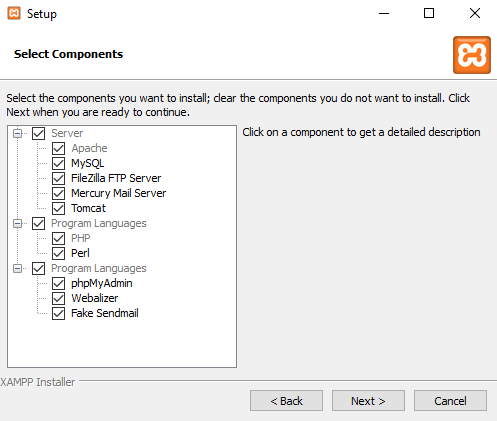
\includegraphics[width=1\textwidth]{/anexos/ManualProgramador/Xampp/1Opciones}
	\caption{\textit{XAMPP}: Servicios que se desean instalar.}
	\label{img:XAMPP_Opciones}
\end{figure}

\begin{figure}[h]
	\centering
	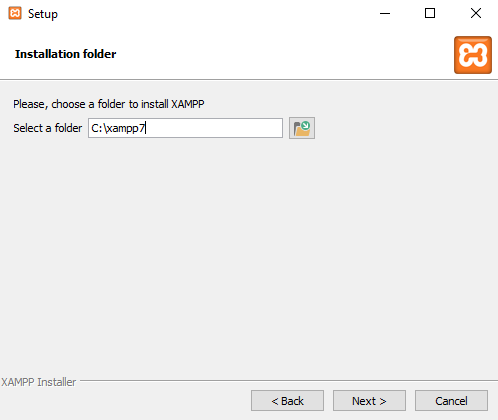
\includegraphics[width=1\textwidth]{/anexos/ManualProgramador/Xampp/2Ruta}
	\caption{\textit{XAMPP}: Ruta donde desplegarlo.}
	\label{img:XAMPP_Ruta}
\end{figure}

Para ver si se ha descargado e instalado correctamente, se puede ejecutar el siguiente comando con el que se mostrará por consola la versión del \textit{PHP} instalado:
\begin{lstlisting}[language=bash]
			php -v
\end{lstlisting}

Los resultados deben de ser como los que se muestran en la figura ~\ref{img:XAMPP_PHP_v}.

\begin{figure}[h]
	\centering
	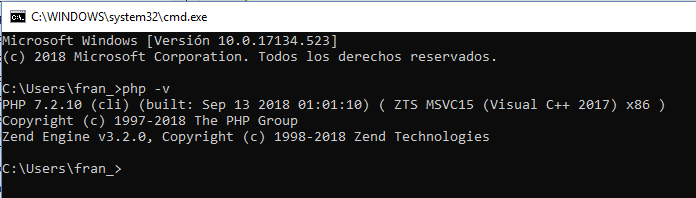
\includegraphics[width=1\textwidth]{/anexos/ManualProgramador/Xampp/3PhpVersion}
	\caption{\textit{XAMPP}: Resultado de ejecutar el comando $php -v$.}
	\label{img:XAMPP_PHP_v}
\end{figure}

Otra de las herramientas que presenta \textit{XAMPP} es un interesante panel de control como el de la figura~\ref{img:XAMPP_Panel}, en el que se podrá iniciar y apagar cada uno de los servicios.

\begin{figure}[h]
	\centering
	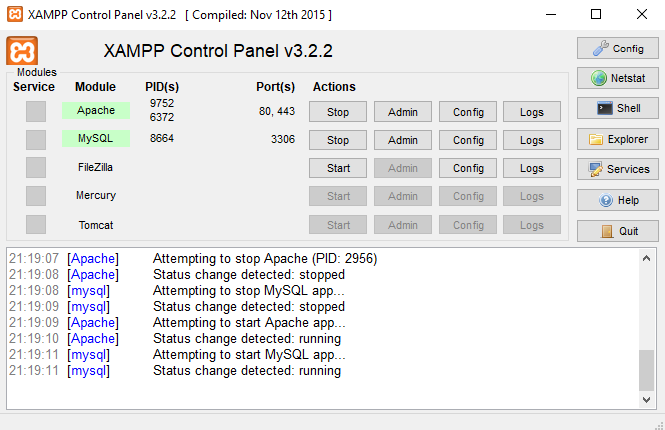
\includegraphics[width=1\textwidth]{/anexos/ManualProgramador/Xampp/4Panel}
	\caption{\textit{XAMPP}: Panel de control con \textit{Apache} y \textit{MySQL} iniciados.}
	\label{img:XAMPP_Panel}
\end{figure}

Si se inicia el servicio de \textit{Apache} correctamente, se puede ver que accediendo a la dirección \href{http://localhost}{localhost}\footnote{\url{http://localhost}} nos muestra información satisfactoria como la de la figura~\ref{img:XAMPP_Correct}.

\begin{figure}[h]
	\centering
	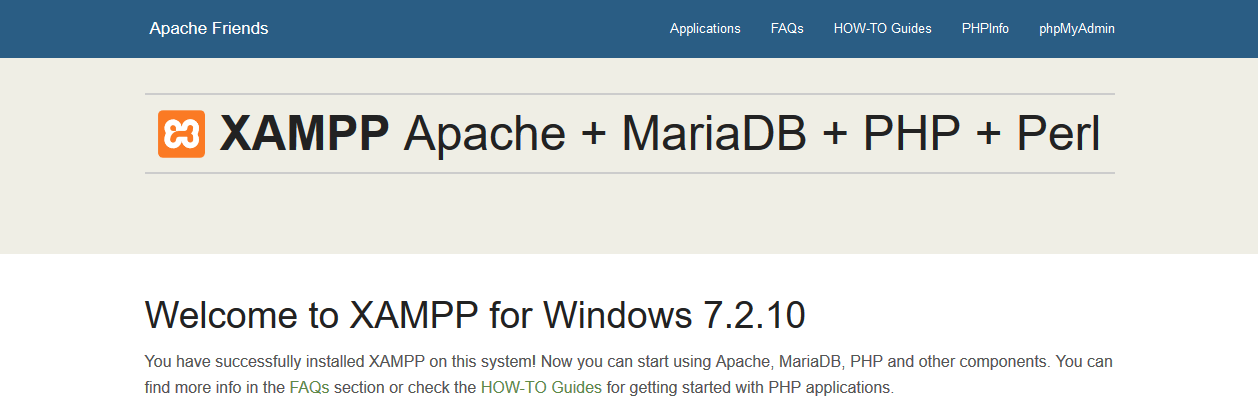
\includegraphics[width=1\textwidth]{/anexos/ManualProgramador/Xampp/5CorrectInstallation}
	\caption{Mensaje de información acerca de que se ha instalado correctamente.}
	\label{img:XAMPP_Correct}
\end{figure}

Con \textit{XAMPP} funcionando, toca configurar las direcciones para indicar donde tenemos nuestro proyecto. Para ello habrá que cambiar alguna linea de código en el fichero de configuración $httpd.conf$ que se encuentra en la ruta \textit{\text{C:/xampp7/apache/conf}}.

Buscamos las lineas: 
\begin{lstlisting}[language=bash]
DocumentRoot "/xampp7/htdocs"
<Directory "/xampp7/htdocs">
\end{lstlisting}
y las cambiamos por la dirección donde hayamos colocado nuestro proyecto, en este caso: 
\begin{lstlisting}[language=bash]
DocumentRoot "C:\Users\fran_\Documents\GitHub\TFG-Instalaciones-Electricas\web\instalaciones_electricas"
<Directory "C:\Users\fran_\Documents\GitHub\TFG-Instalaciones-Electricas\web\instalaciones_electricas">
\end{lstlisting}

De esta manera, ya no redireccionará a la página anterior sino que cogerá la ruta especificada.

Aunque lo que se va a comentar a continuación no es obligatorio, si que es aconsejable pues si se desea tener varios proyectos, es incómodo trabajar con la dirección \textit{localhost} pues tendríamos que andar modificando estos archivos continuamente. Para ello existe la posibilidad de configurar todos los \textit{virtual hosts} que se deseen. Esto significa que se podrán dar direcciones concretas a cada uno de los proyectos. Para ello, se descomentará la siguiente linea:

\begin{lstlisting}[language=bash]
# Virtual hosts
Include conf/extra/httpd-vhosts.conf
\end{lstlisting}

El siguiente paso es dirigirse al fichero $httpd-vhosts.conf$ que se encuentra en el directorio \textit{\text{C:/xampp7/apache/conf/extra}} para colocar las siguientes lineas al final del archivo y crear un primer \textit{virtual hosts}.

\begin{lstlisting}[language=bash]
<VirtualHost *:80>
DocumentRoot "C:\Users\fran_\Documents\GitHub\TFG-Instalaciones-Electricas\web\instalaciones_electricas\webroot"
ServerName instalaciones_electricas.fsg
<Directory "C:\Users\fran_\Documents\GitHub\TFG-Instalaciones-Electricas\web\instalaciones_electricas\webroot">
Require all granted
</Directory>
</VirtualHost>
\end{lstlisting}

\begin{itemize}
\item \textit{DocumentRoot}: Aquí se indica la ruta del proyecto hasta la carpeta \textit{webroot} que como se ha explicado antes es la parte pública, la que tiene acceso el usuario.
\item \textit{ServerName}: Dirección url para ese proyecto.
\end{itemize}

Cabe destacar que siempre que se modifique cualquier fichero de configuración se tendrán que reiniciar los servicios afectados, por lo que a continuación, el último paso será acceder de nuevo al panel de control~\ref{img:XAMPP_Panel} y reiniciar el servicio.

Por último, lo que queda de configurar es la base de datos \textit{MySQL}. Aunque con el paquete \textit{XAMPP} viene preparado para su uso \textit{phpMyAdmin}, se ha decidido descargar \href{https://www.heidisql.com/download.php}{\textit{HeidiSQL}}\footnote{\textit{HeidiSQL}: \url{https://www.heidisql.com/download.php}} pues presenta una interfaz más amigable y estable. Ademas, existe una versión portable que no requiere de instalación.

Si ejecutamos la aplicación, aparecerá una pantalla como la de la figura~\ref{img:Heidi}, donde nos aparecerán todas las sesiones que tengamos activas:

\begin{figure}[h]
	\centering
	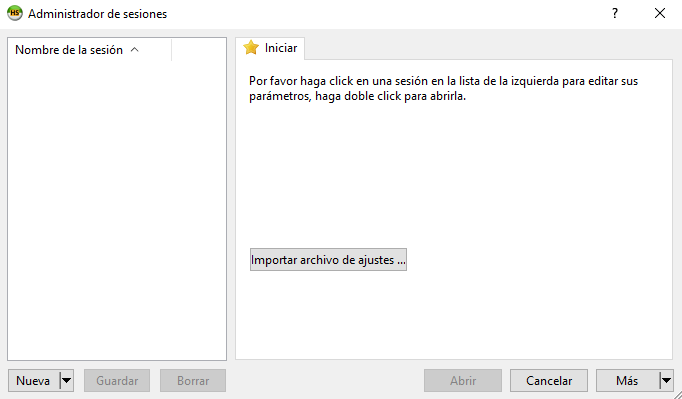
\includegraphics[width=1\textwidth]{/anexos/ManualProgramador/Xampp/8Heidi}
	\caption{Pantalla de inicio de \textit{HeidiSQL}.}
	\label{img:Heidi}
\end{figure}

Procedemos a crear una nueva sesión con los parámetros que se ven en la figura~\ref{img:Heidi_2}:

\begin{figure}[h]
	\centering
	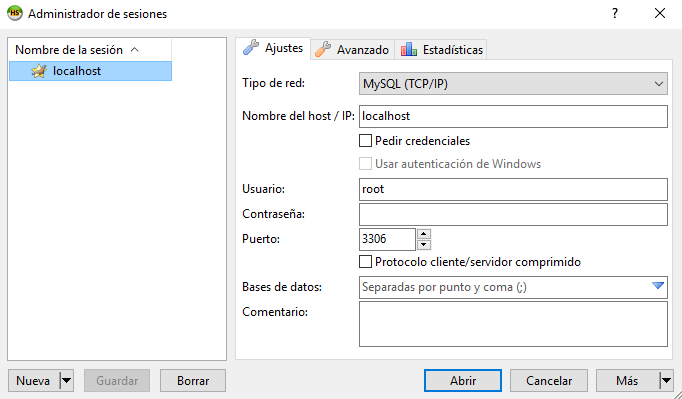
\includegraphics[width=1\textwidth]{/anexos/ManualProgramador/Xampp/9Heidi_2}
	\caption{Parámetros para una nueva sesión en entorno local.}
	\label{img:Heidi_2}
\end{figure}

Con la sesión ya creada, se podrá crear una base de datos nueva con las tabas que se desee. A continuación, en la figura~\ref{img:Heidi_3} se va a mostrar como crear un usuario para esa base de datos para que posteriormente se pueda enlazar con el proyecto. 

\begin{figure}[h]
	\centering
	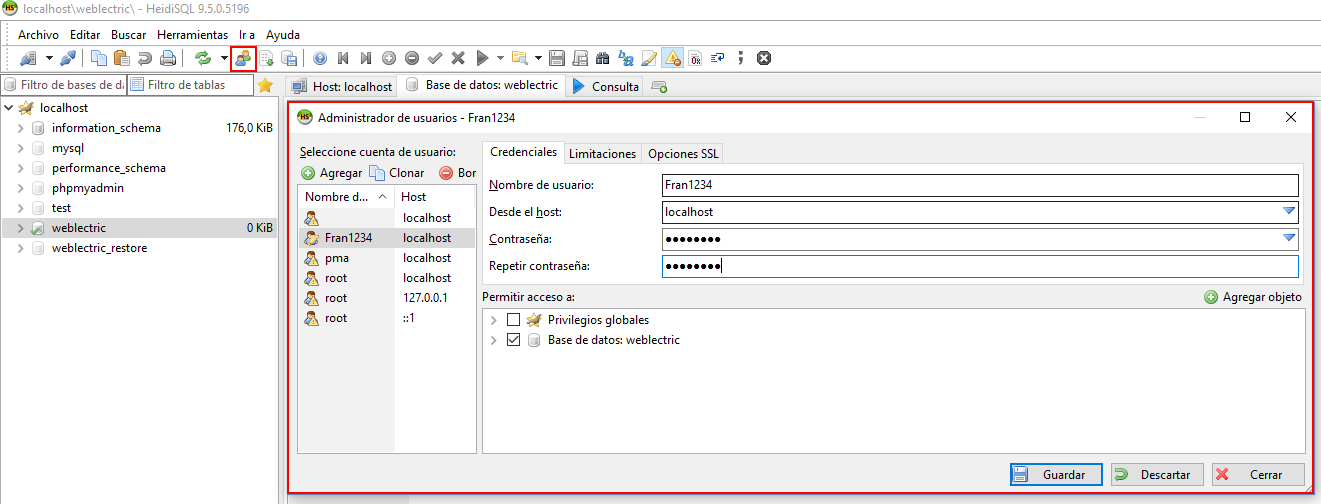
\includegraphics[width=1\textwidth]{/anexos/ManualProgramador/Xampp/10Heidi_3}
	\caption{Parámetros para asociar un usuario a la base de datos.}
	\label{img:Heidi_3}
\end{figure}

\newpage


\section{Compilación, instalación y ejecución del proyecto}

En primer lugar, se procederá a descargar \href{https://github.com/fransaiz95/Weblectric2018}{\textit{Weblectric}}\footnote{\textit{Weblectric}: \url{https://github.com/fransaiz95/Weblectric2018}} del repositorio de \textit{GitHub}.

El lugar en el que se descomprimirá el archivo descargado, será el directorio que se haya especificado anteriormente, en nuestro caso:
\begin{lstlisting}[language=bash]
C:\Users\fran_\Documents\GitHub\TFG-Instalaciones-Electricas\web\"
\end{lstlisting}

Como se puede ver en la figura~\ref{img:XAMPP_Finish}, si ahora se introduce la url que se ha establecido en el \textit{virtual host}, se accederá satisfactoriamente a la pantalla principal del proyecto.

\begin{figure}[h]
	\centering
	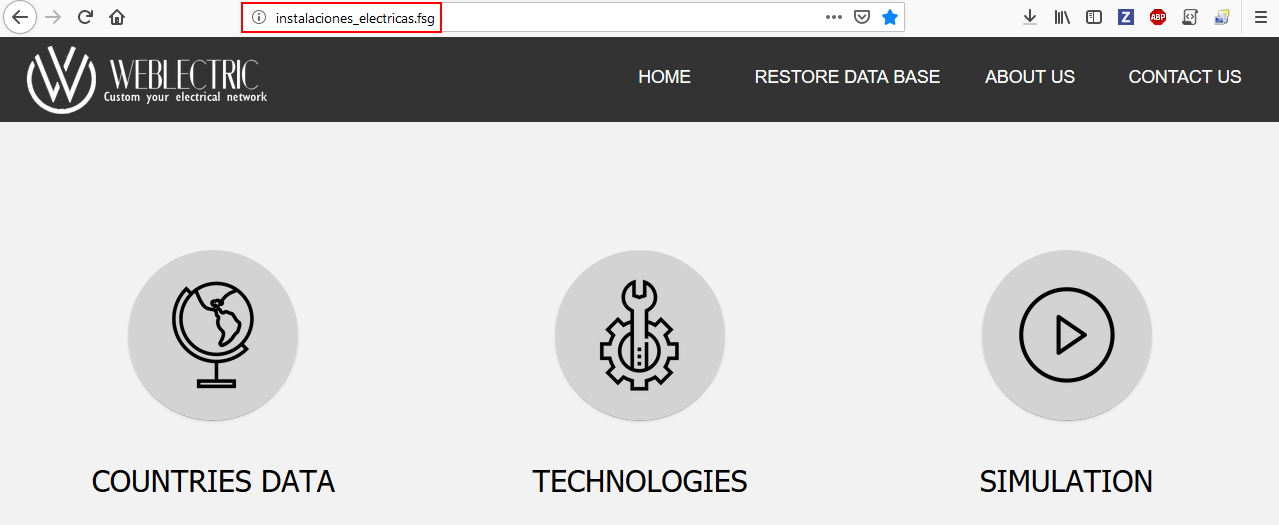
\includegraphics[width=1\textwidth]{/anexos/ManualProgramador/Xampp/6Finish}
	\caption{\textit{Virtual host} correctamente configurado.}
	\label{img:XAMPP_Finish}
\end{figure}

Dentro del entorno de desarrollo, no hay dificultades pues no hay más que abrir la carpeta contenedora del proyecto.

En este proyecto, que se ha utilizado \textit{Visual Studio Code} como herramienta para desarrollar, la estructura viene representada de la siguiente manera: ~\ref{img:VsCodeWeblectric}

\begin{figure}[h]
	\centering
	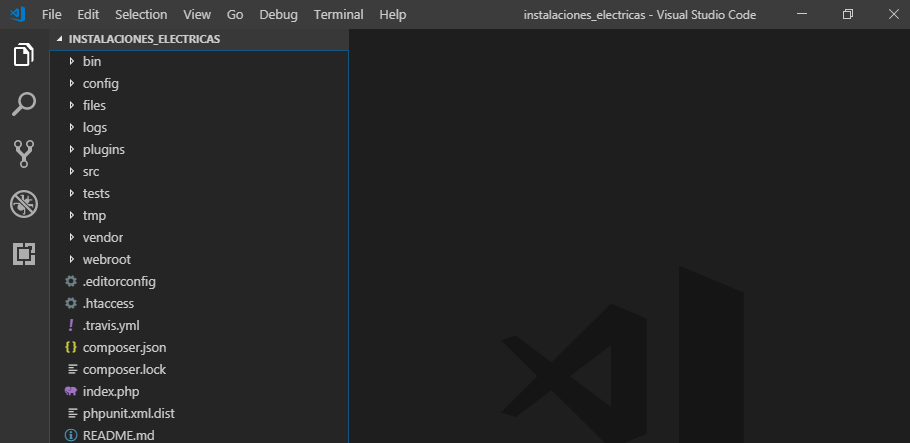
\includegraphics[width=0.8\textwidth]{/anexos/ManualProgramador/Xampp/7VscodeWeblectric}
	\caption{Estructura de directorios con el proyecto importado.}
	\label{img:VsCodeWeblectric}
\end{figure}

\newpage

Para acabar, en el archivo $app.conf$ que se encuentra dentro de la carpeta $config$ es necesario reemplazar las lineas que a continuación se van a describir para enlazar el proyecto con la base de datos:

\begin{lstlisting}[language=php]
'Datasources' => [
	'default' => [
		'className' => 'Cake\Database\Connection',
		'driver' => 'Cake\Database\Driver\Mysql',
		'persistent' => false,
		'host' => 'localhost',
		'username' => 'Fran1234',
		'password' => 'Fran1234',
		'database' => 'weblectric',
		'encoding' => 'utf8',
		'timezone' => 'UTC',
		'flags' => [],
		'cacheMetadata' => true,
		'log' => false,
	],
],
\end{lstlisting}





\apendice{Documentación de usuario}

\section{Introducción}

\section{Requisitos de usuarios}

\section{Instalación}

\section{Manual del usuario}





\bibliographystyle{plain}
\bibliography{bibliografiaAnexos}

\end{document}
